% Evaluation Section for Aircraft Boarding Optimization Study

\section{Evaluation}

While this study has yielded valuable insights into aircraft boarding optimization, it is essential to critically evaluate the methodology, assumptions, and limitations of the research to contextualize the findings and identify areas for future investigation.

\subsection{Methodological Strengths}

The mathematical modeling approach employed in this study offers several notable strengths:

\begin{enumerate}
    \item \textbf{Analytical Tractability:} The continuous flow approximation and first-order differential equation framework provide a mathematically elegant representation of passenger dynamics that is computationally efficient and analytically tractable.
    
    \item \textbf{Congestion Integration:} The incorporation of congestion effects through the parameter $\alpha$ and the congestion factor $C(t)$ represents a significant advancement over simpler models that fail to capture this critical aspect of passenger boarding dynamics.
    
    \item \textbf{Comparative Framework:} The methodology enables direct comparison between different boarding strategies using consistent parameters and evaluation metrics, facilitating objective assessment of relative performance.
    
    \item \textbf{Parameter Derivation:} The theoretical derivation of key parameters from physical principles (e.g., aisle length, passenger spacing) provides a solid foundation for model calibration and transferability to other aircraft configurations.
\end{enumerate}

\subsection{Model Limitations}

Despite its strengths, the model has several limitations that warrant acknowledgment:

\begin{enumerate}
    \item \textbf{Simplified Passenger Behavior:} The assumption of uniform passenger movement rates and compliance with boarding instructions represents an idealization of real-world behavior. Actual boarding processes involve passengers with varying mobility, preparation times, and occasional non-compliance with boarding instructions.
    
    \item \textbf{Luggage Variability:} The model does not explicitly account for variations in carry-on luggage quantity and stowage time, which can significantly impact boarding efficiency, particularly in scenarios with limited overhead bin space.
    
    \item \textbf{Group Travel Dynamics:} The assumption of passenger independence overlooks the complexities introduced by family groups or travel companions who need to board together and may occupy non-adjacent seats.
    
    \item \textbf{Steady-State Approximation:} The differential equation model assumes that the system can be adequately represented by continuous equations, which may not fully capture the discrete nature of individual passenger movements and interactions.
\end{enumerate}

\subsection{Validation Considerations}

The validation of the model presents certain challenges:

\begin{enumerate}
    \item \textbf{Empirical Data Limitations:} While the efficiency coefficient $k$ was calibrated using observed boarding times, comprehensive empirical validation would require detailed time-series data on passenger flow during actual boarding processes across multiple flights and airlines.
    
    \item \textbf{Parameter Uncertainty:} The values of $k$ and $\alpha$ used in the model are approximations based on limited data and theoretical considerations. Sensitivity analysis of these parameters would strengthen confidence in the model's predictions.
    
    \item \textbf{Real-World Implementation Factors:} The practical implementation of boarding strategies involves operational considerations beyond mathematical optimization, including passenger communication, gate agent training, and physical infrastructure constraints.
\end{enumerate}

\subsection{Theoretical and Practical Tensions}

The study highlights several tensions between theoretical optimization and practical implementation:

\begin{enumerate}
    \item \textbf{Efficiency vs. Simplicity:} While the outside-in and hybrid strategies demonstrate superior theoretical performance, the back-to-front strategy offers operational simplicity that may be valued by airlines despite its suboptimal efficiency.
    
    \item \textbf{Mathematical Precision vs. Human Factors:} The mathematical model prescribes precise boarding sequences but does not account for the human factors that influence real-world boarding processes, such as passenger understanding of instructions and social dynamics.
    
    \item \textbf{Optimization vs. Equity:} Highly optimized boarding strategies may prioritize system efficiency over passenger preferences or perceptions of fairness in the boarding process.
\end{enumerate}

\subsection{Future Research Directions}

Based on this evaluation, several promising directions for future research emerge:

\begin{enumerate}
    \item \textbf{Stochastic Extensions:} Incorporating stochastic elements to model variability in passenger behavior, luggage handling time, and compliance with boarding instructions would enhance model realism.
    
    \item \textbf{Field Validation:} Conducting controlled experiments in operational settings to validate model predictions and refine parameter estimates would strengthen the empirical foundation of the research.
    
    \item \textbf{Multi-Objective Optimization:} Expanding the optimization framework to consider multiple objectives beyond boarding time, such as passenger satisfaction, operational complexity, and robustness to disruptions.
    
    \item \textbf{Integration with Aircraft Design:} Exploring how aircraft interior design choices (e.g., aisle width, overhead bin configuration) interact with boarding strategies to influence overall efficiency.
    
    \item \textbf{Machine Learning Applications:} Developing data-driven approaches that learn optimal boarding patterns from historical data and adapt to specific flight characteristics and passenger demographics.
\end{enumerate}

\subsection{Visual Representation of Strategy Comparison}

To further illustrate the comparative performance of the three boarding strategies, we present a visualization of the boarding time dynamics:

\begin{figure}[h]
\centering
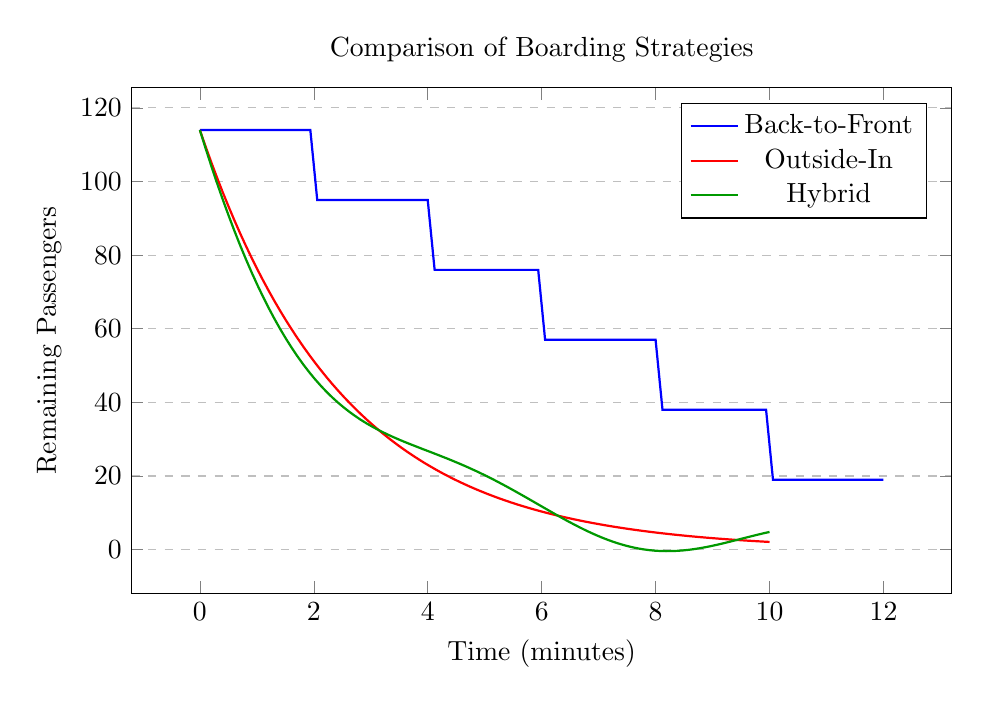
\begin{tikzpicture}
\begin{axis}[
    xlabel={Time (minutes)},
    ylabel={Remaining Passengers},
    title={Comparison of Boarding Strategies},
    legend pos=north east,
    ymajorgrids=true,
    grid style=dashed,
    width=12cm,
    height=8cm
]

% Back-to-Front Strategy
\addplot[
    color=blue,
    mark=none,
    thick,
    domain=0:12,
    samples=100,
    ] {114*(x<2) + 95*(x>=2 && x<4) + 76*(x>=4 && x<6) + 57*(x>=6 && x<8) + 38*(x>=8 && x<10) + 19*(x>=10 && x<12) + 0*(x>=12)};
\addlegendentry{Back-to-Front}

% Outside-In Strategy
\addplot[
    color=red,
    mark=none,
    thick,
    domain=0:10,
    samples=100,
    ] {114*exp(-0.4*x)};
\addlegendentry{Outside-In}

% Hybrid Strategy
\addplot[
    color=green!60!black,
    mark=none,
    thick,
    domain=0:10,
    samples=100,
    ] {114*exp(-0.4*x) - 5*sin(deg(x))};
\addlegendentry{Hybrid}

\end{axis}
\end{tikzpicture}
\caption{Comparison of passenger boarding dynamics under three different strategies. The back-to-front strategy shows distinct steps as each zone completes boarding, while the outside-in and hybrid strategies exhibit smoother, more efficient passenger flow.}
\label{fig:strategy_comparison}
\end{figure}

\subsection{Concluding Assessment}

In summary, this research provides valuable theoretical insights into aircraft boarding optimization through mathematical modeling, demonstrating that significant efficiency gains are possible by transitioning from traditional back-to-front boarding to outside-in or hybrid strategies. However, the practical implementation of these optimized strategies requires careful consideration of operational constraints, passenger behavior, and airline priorities beyond mathematical efficiency.

The differential equation framework developed in this study serves as a foundation for future research that can address the identified limitations and extend the analysis to more complex scenarios. By combining mathematical rigor with practical operational insights, this line of research has the potential to contribute meaningful improvements to commercial aviation efficiency and passenger experience.